
% ---------------------------------------------------
%
% Trabajo de Fin de Grado. 
% Author: Alejandro Hernández Padrón. 
% Capítulo: La aplicación ULL-AR. 
% Fichero: Cap4_TheApplication.tex
%
% ----------------------------------------------------
%

\chapter{La aplicación ULL-AR} \label{chap:LaAplicacion} 

En este capítulo explicaremos la aplicación ULL-AR utilizando la especificación de requisitos de esta y explicando su funcionamiento.

\section{Especificación de requisitos} % (fold)

Nos dispondremos a exponer los requisitos de la presente aplicación propuesta para el desarrollo de este TFG.

Se trata de una aplicación para móviles, más concretamente, a aquellos dispositivos que utilizan Android como sistema operativo. Es una aplicación diseñada para los estudiantes de la Universidad de La Laguna, la cual les permita ubicarse, detectar y reconocer las instalaciones y edificios pertenecientes a la universidad, mediante técnicas de realidad aumentada basadas en la geolocalización.

Los requisitos principales de la aplicación son:
\begin{itemize}
    \item La aplicación se desarrollará para dispositivos con Android. Se utilizará Android Studio como IDE para su desarrollo.
    \item Se implementarán técnicas de realidad aumentada basadas en la geolocalización para mostrar al usuario la instalación de la ULL a la cual apunte con la cámara.
    \item Las instalaciones, junto a su información correspondiente, estarán ubicadas en un base datos en la nube. El servidor que se conecte con esta base de datos también deberá estar en la nube.
\end{itemize}

\section{Especificación detallada de los requisitos} 

La aplicación se iniciará una Splash Screen \cite{URL::SplashScreen} o pantalla de inicio con el logo de la Universidad de La Laguna. Esta pantalla dará paso a una ventana de login.

Para poder utilizar la aplicación, el usuario ha de ser alumno de la Universidad de La Laguna y poseer su respectiva cuenta de Google con el correo institucional de la ULL. Este correo ha de tener el siguiente formato: ``\textit{aluxxxxxxxxxx@ull.edu.es}''. Sin ella no se podrá acceder a la aplicación. Además, se podrá cerrar la sesión de esta cuenta.

Una vez logueado accederemos a una ventana de \textit{Inicio} en la que aparecerá un acceso directo a las ventanas de \textit{Mapa ULL} y \textit{Navegación en modo RA} que explicaremos más adelante. A su vez, dispondrá de los accesos directos a enlaces de interés de Universidad de La Laguna que se abrirán en un navegador externo.

Una vez dentro de la aplicación, tendremos un menú para movernos por las diferentes ventanas. Se utilizará un menú deslizante lateral o \textit{Navigation Drawer} \cite{URL::NavigationDraw} ubicado en la parte superior izquierda de la aplicación. Este menú deberá ser simple e intuitivo.

Como accesos en este menú disponemos de las siguientes ventanas:

\begin{itemize}
    \item Inicio. Ventana inicial con la que se abre la aplicación.
    \item Mapa ULL. Esta ventana contendrá un mapa de la universidad con todas las instalaciones en la base de datos. 
    \item Navegación en modo RA. En esta ventana, mediante el uso de la cámara, se identificarán las instalaciones universitarias a los que el usuario apunte y permitirá mostrar una pestaña con información detallada de las mismas.
    \item instalaciones de la ULL. Contiene todas la ubicaciones e instalaciones de la Universidad de La Laguna y permitirá la búsqueda de estas. 
    \item Configuración. Permitirá acceder a los ajustes de la aplicación.
    \item Cerrar cesión. Cerrará la sesión actual y nos devolverá a la ventana de login.
    \item Info. Información de aplicación así como de su autor.
\end{itemize}

Cada instalación de la universidad tendrá una ficha de información que será accesible desde una ventana de la aplicación con la siguiente información:

\begin{itemize}
    \item \textbf{Id}: campo para identificar la instalación.
    \item \textbf{Nombre}: nombre oficial de la instalación.
    \item \textbf{Ubicación}: la ubicación exacta en la que se encuentra la instalación. 
    \item \textbf{Descripción}: descripción de la instalación con el objetivo y actividades que se desarrollan en él.
    \item \textbf{Imagen}: imagen de la instalación.
    \item \textbf{Lista de enlaces de interés}: una lista con los enlaces a las instituciones, servicios, departamentos y grados que se imparten en esta instalación.
\end{itemize}

Esta información estará guardada en una base de datos en la nube. Para acceder a esta, se dispondrá de un servidor en la nube que conecte con la base de datos y envié la información a la aplicación.

\section{Ventanas de la aplicación}

Nada más iniciar la aplicación nos encontramos con dos ventanas.

\begin{figure}[h]
\hspace*{\fill}%
\begin{subfigure}[h]{0.32\linewidth}

\includegraphics[width=\linewidth]{splashApp}
\caption{Splash-Screen.}
\label{fig:splashApp}
\end{subfigure}
\hfill%
\begin{subfigure}[h]{0.32\linewidth}
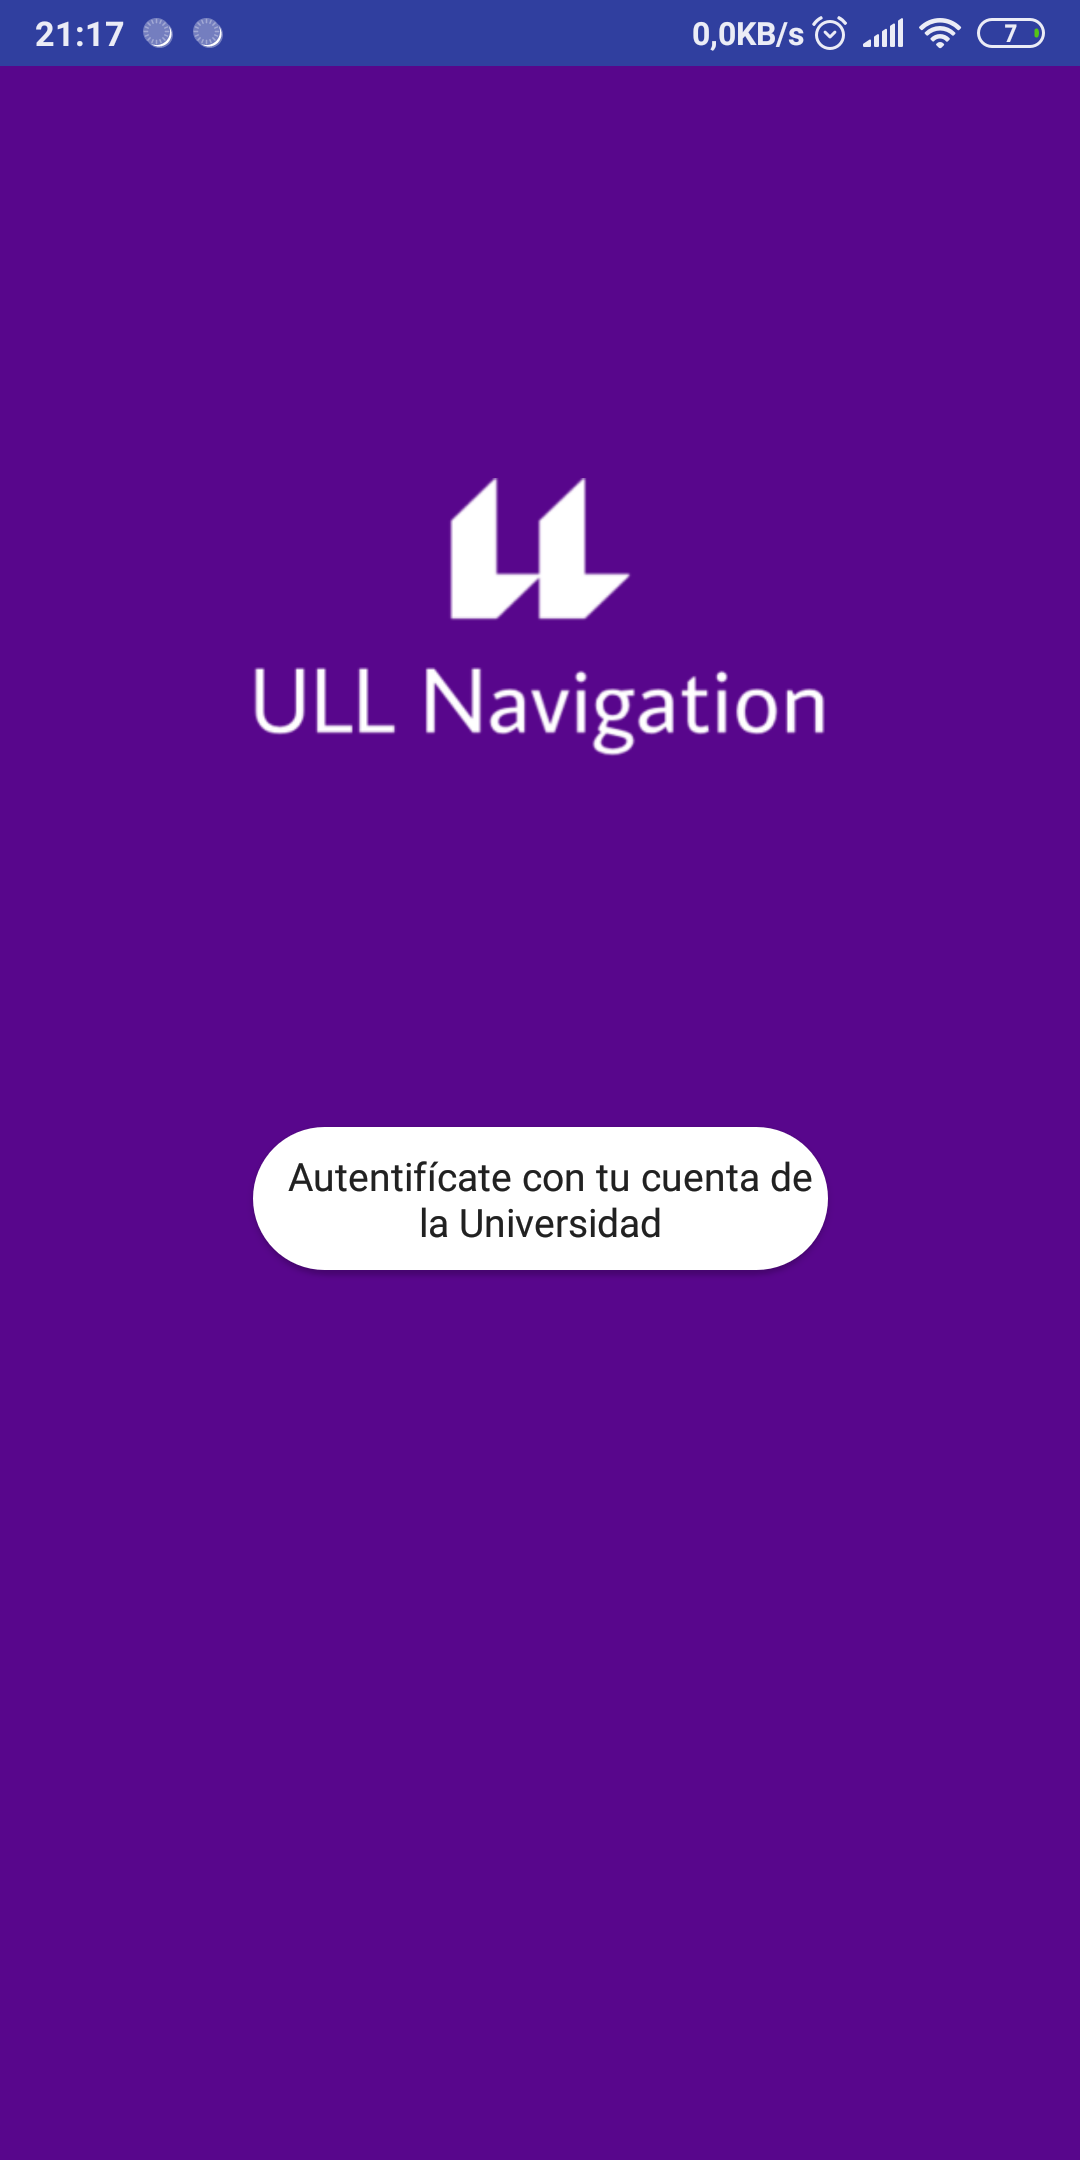
\includegraphics[width=\linewidth]{loginApp}
\caption{Login.}
\label{fig:loginApp} 
\end{subfigure}%
\caption{Ventanas de iniciales de \textit{ULL-AR}.}
\hspace*{\fill}%
\end{figure}
  
La primera ventana (véase Figura \ref{fig:splashApp}) es la pantalla de inicio o Splash Screen que aparece cuando ejecutamos la aplicación. Tras unos segundos, se carga la ventana de \textit{Login} (véase Figura \ref{fig:loginApp}). Para poder loguearnos deberemos tener una cuenta de Google de la ULL. Una vez que presionamos en el botón del medio, se nos abrirá una ventana de diálogo para que pongamos nuestra cuenta.

Cuando nos hayamos logueado con éxito, se nos abrirá la venta de \textit{Inicio} (véase Figura \ref{fig:homeApp}). En esta tendremos una lista de accesos directos a las funcionalidades principales de la aplicación, como son \textit{Navegación en modo RA}, \textit{Mapa ULL} y una serie de enlaces a sitios web relacionados con la ULL.

\begin{figure}[h]
    \hspace*{\fill}%
    \begin{subfigure}[h]{0.35\linewidth}
    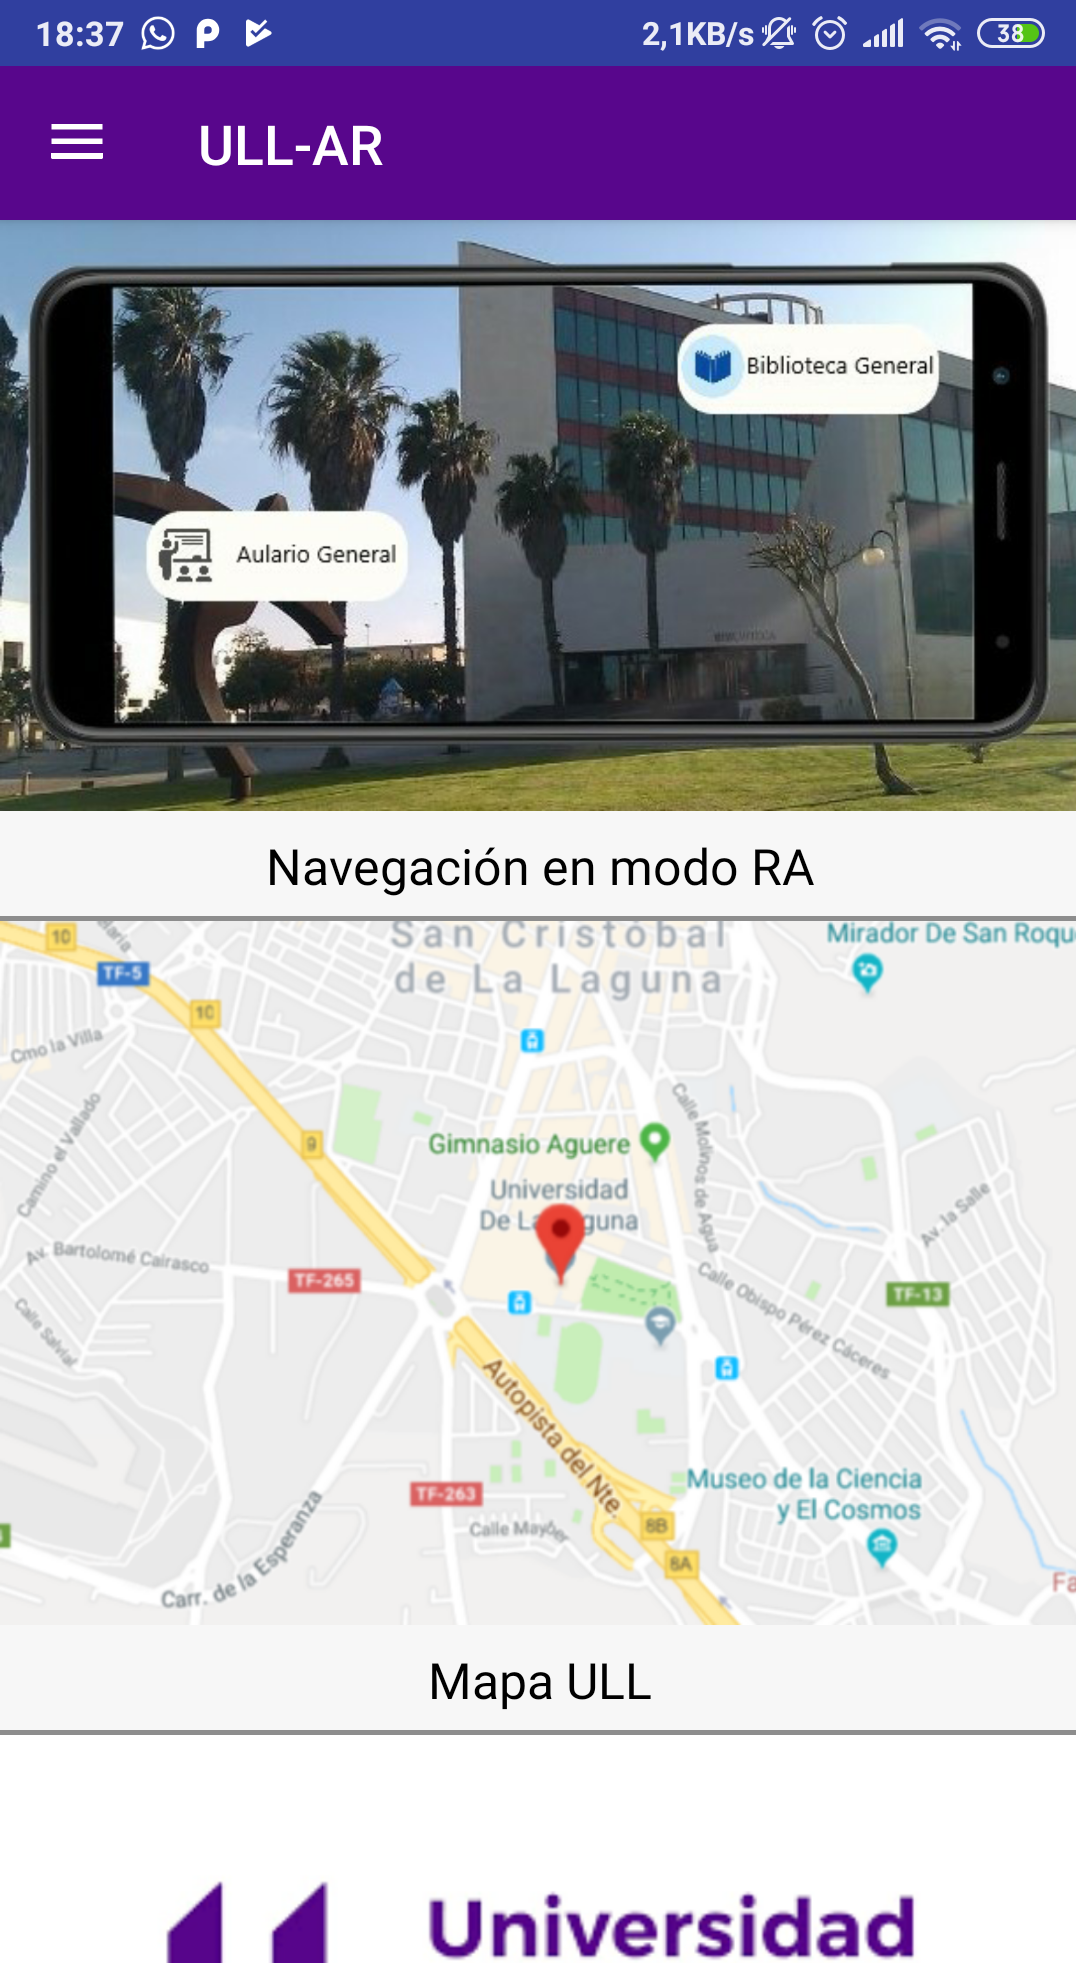
\includegraphics[width=\linewidth]{homeApp}
    \caption{Inicio.}
    \label{fig:homeApp}
    \end{subfigure}
    \hfill%
    \begin{subfigure}[h]{0.35\linewidth}
    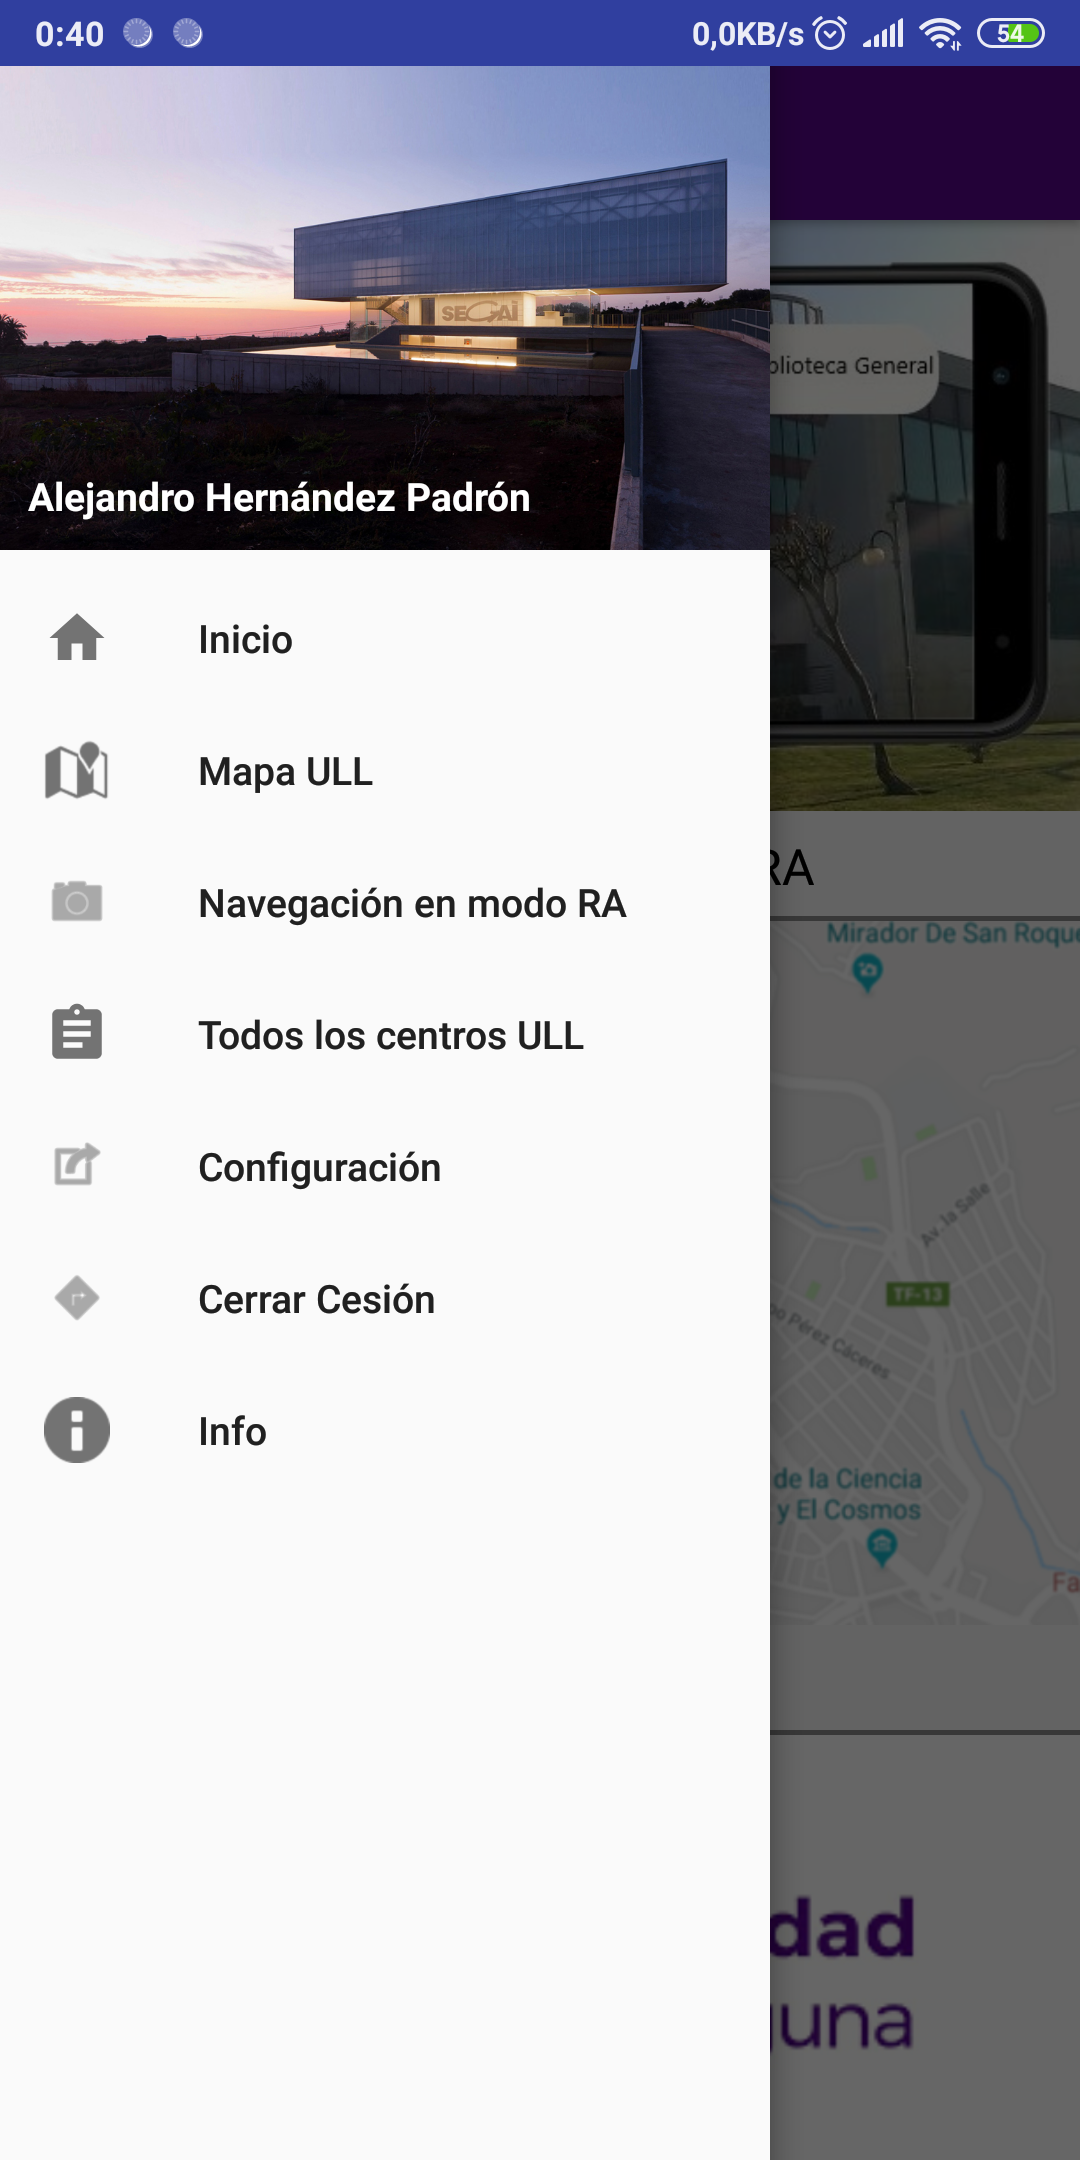
\includegraphics[width=\linewidth]{menuApp}
    \caption{Menu. Navigation Drawer.}
    \label{fig:menuApp}
    \end{subfigure}%
    \caption{Ventana \textit{Inicio} y el \textit{Menú} de \textit{ULL-AR}.}
    \hspace*{\fill}%
\end{figure}

En la esquina superior izquierda de aplicación tenemos el acceso al menú \textit{Navigation Drawer}. Si lo pulsamos se nos desplegará el menú que nos permite movernos por las distintas ventanas de la aplicación (véase Figura \ref{fig:menuApp}).

Si nos movemos a la ventana de \textit{Mapa ULL} (véase Figura \ref{fig:mapsApp}) veremos el mapa de la API de Google Maps. En este mapa nos aparecerán en pines azules las ubicaciones con sus respectivos nombres de la ULL que están guardadas en la base de datos. Cuando el GPS del dispositivo encuentre la ubicación aparecerá un pin rojo que indicará nuestra posición. En la parte de abajo en el centro disponemos de un botón llamado ``AR Mode'' que nos llevará directo a la ventana de \textit{Navegación en modo RA}.
  
\begin{figure}[h]
    \centering
    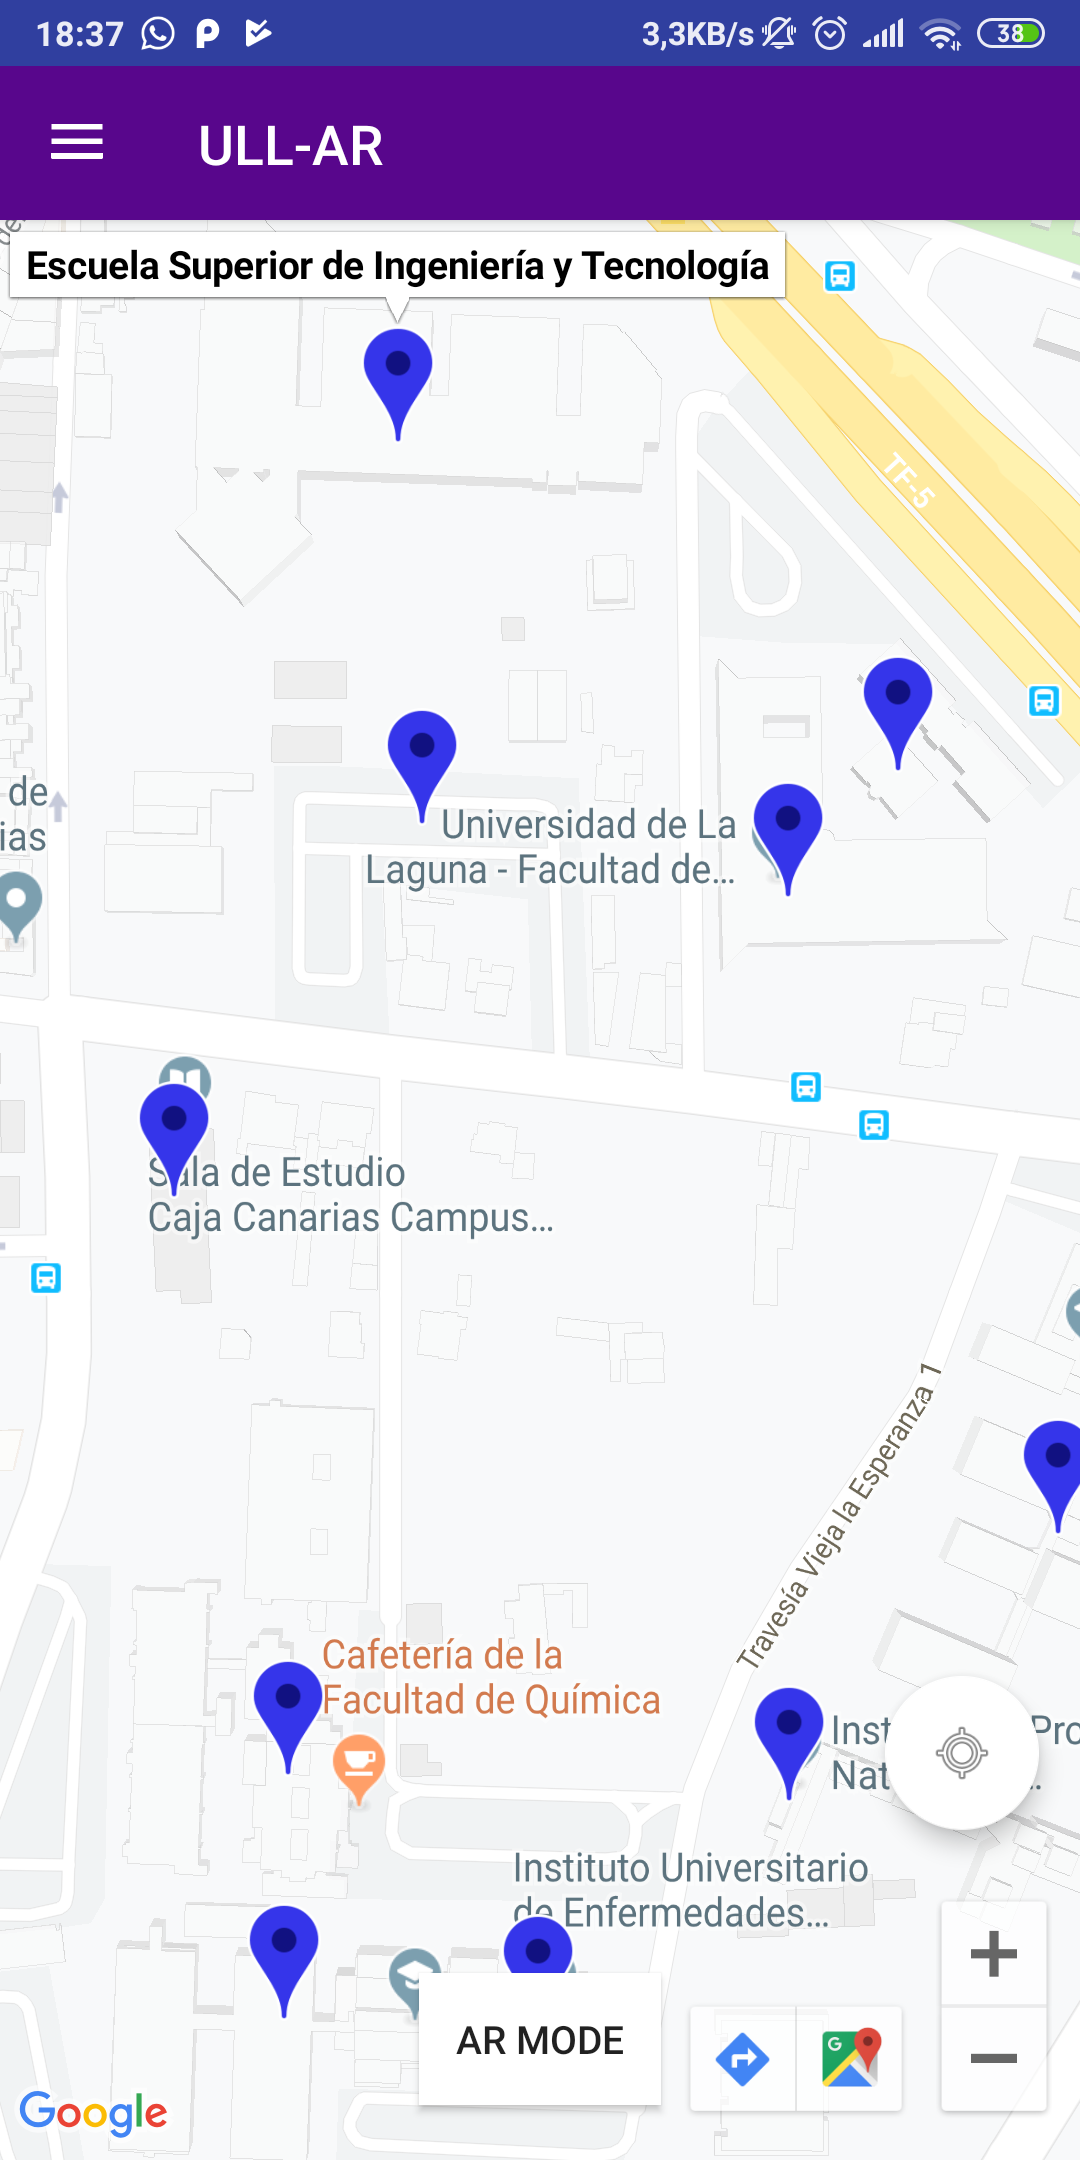
\includegraphics[width=0.38\linewidth]{mapsApp}
    \caption{Mapa ULL.}
    \label{fig:mapsApp}
\end{figure}

En la ventana de \textit{Navegación en modo RA} se nos mostrará la vista de la cámara de nuestro dispositivo 

XXX

% \begin{figure}[h]
%     \hspace*{\fill}%
%     \begin{subfigure}[h]{0.35\linewidth}
%     \includegraphics[width=\linewidth]{App}
%     \caption{Ventana de \textit{Inicio}}
%     \label{fig:homeApp}
%     \end{subfigure}
%     \hfill%
%     \begin{subfigure}[h]{0.35\linewidth}
%     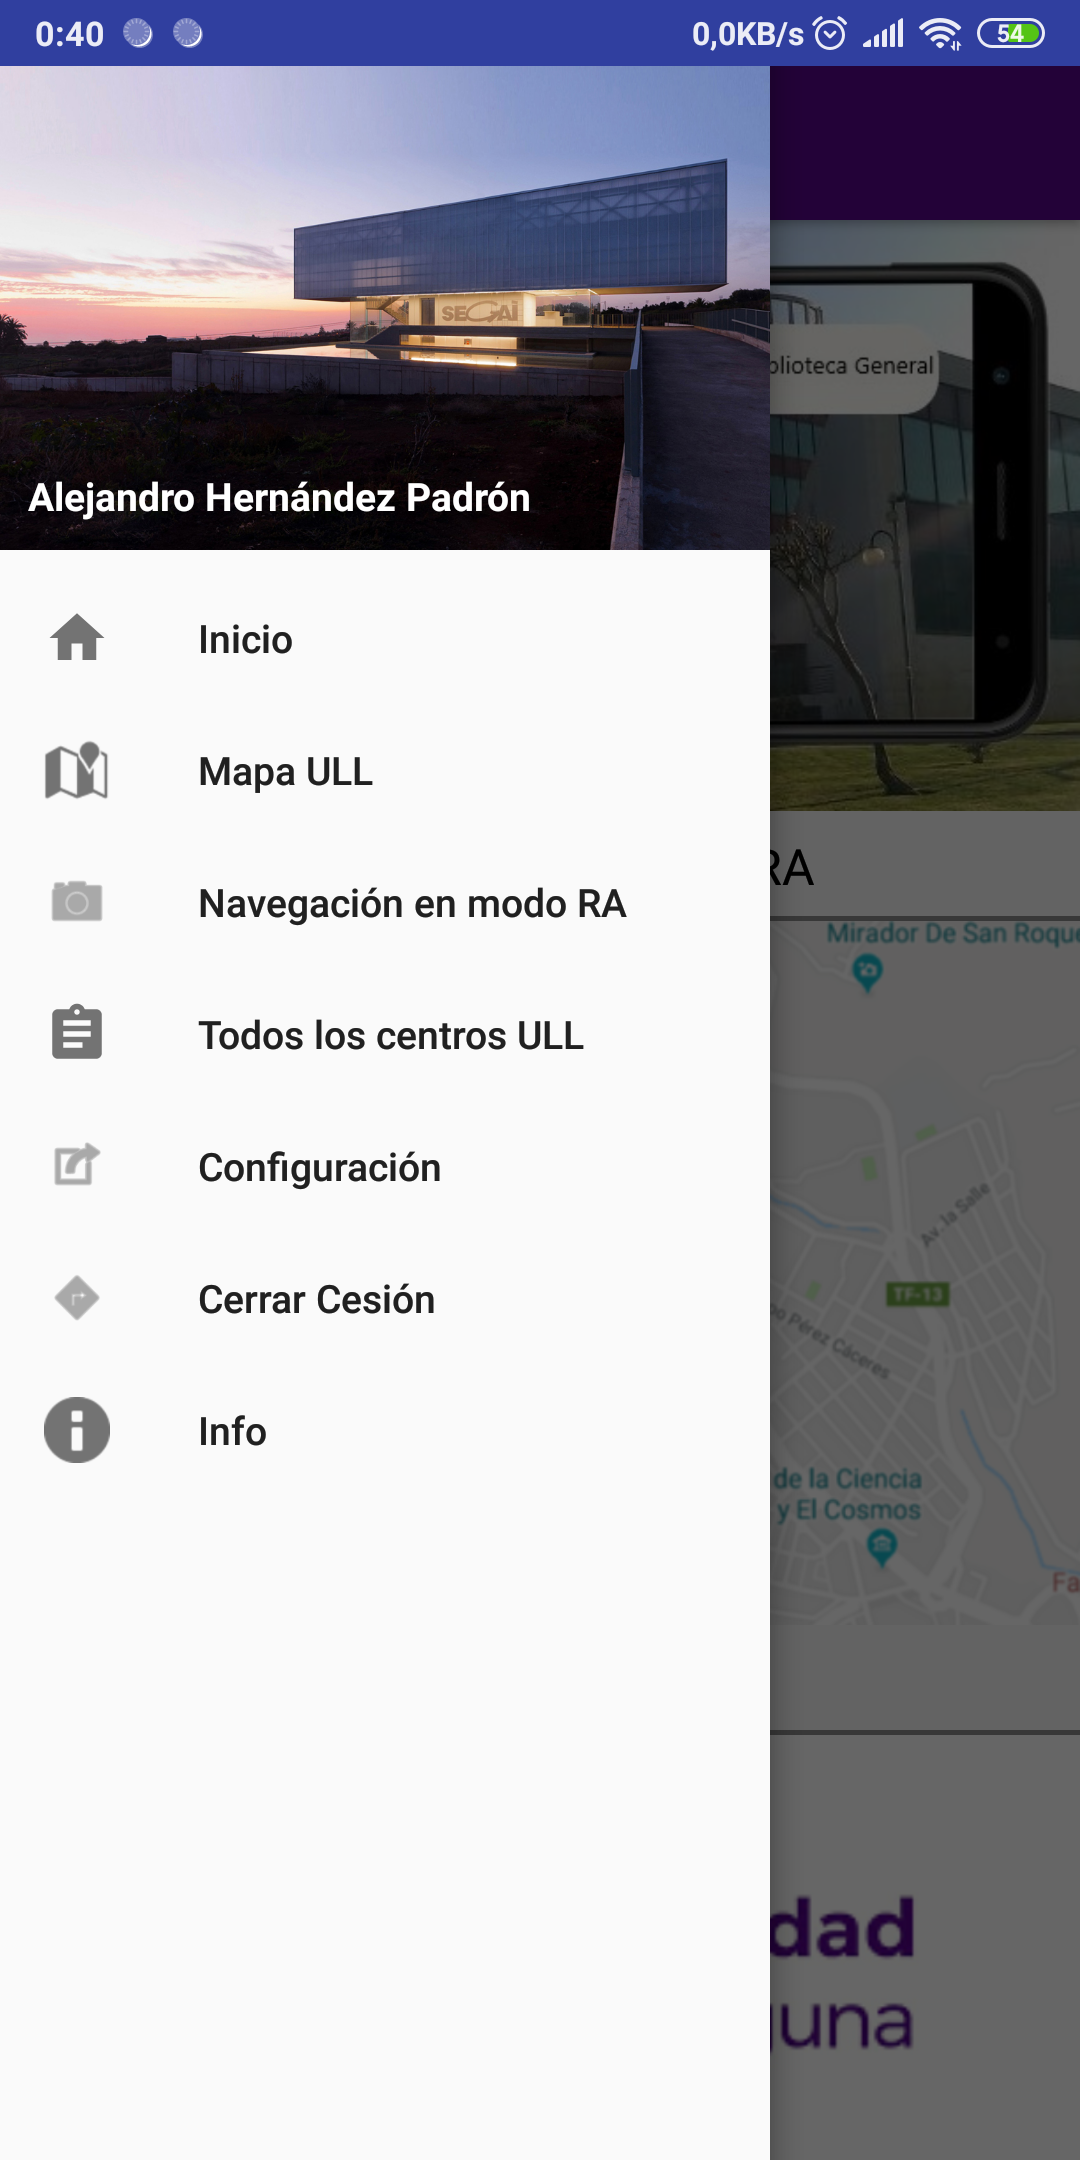
\includegraphics[width=\linewidth]{menuApp}
%     \caption{Ventana de \textit{Inicio}}
%     \label{fig:menuApp}
%     \end{subfigure}%
%     \caption{Ventana Inicio y menú de \textit{ULL-AR}}
%     \hspace*{\fill}%
% \end{figure}

A través del menú de la aplicación podemos acceder a la ventana de \textit{Todas las instalaciones ULL} (véase Figura \ref{fig:allSitesApp}). Aquí se nos mostrarán todas las instalaciones de la ULL que se encuentran en la base de datos. Se podrá hacer una búsqueda de cualquier instalación en la barra superior de la aplicación. Si pulsamos cualquiera de estas instalaciones se nos desplegará una ventana con la información detallada de la instalación.

En la ventana \textit{Información de la instalación} (véase Figura \ref{fig:siteInfoApp}) se dispondrá la información de esta. Aquí se nos mostrará una imagen de este, nombre y descripción de la instalación y una lista de enlaces con los servicios, secretarias, grados y departamentos que podemos encontrar. Disponemos de un botón en la parte inferior de la imagen de la instalación que nos abrirá la ruta a su ubicación en la aplicación de Google Maps para poder llegar a ella.  
 
\begin{figure}[h]
    \hspace*{\fill}%
    \begin{subfigure}[h]{0.35\linewidth}
    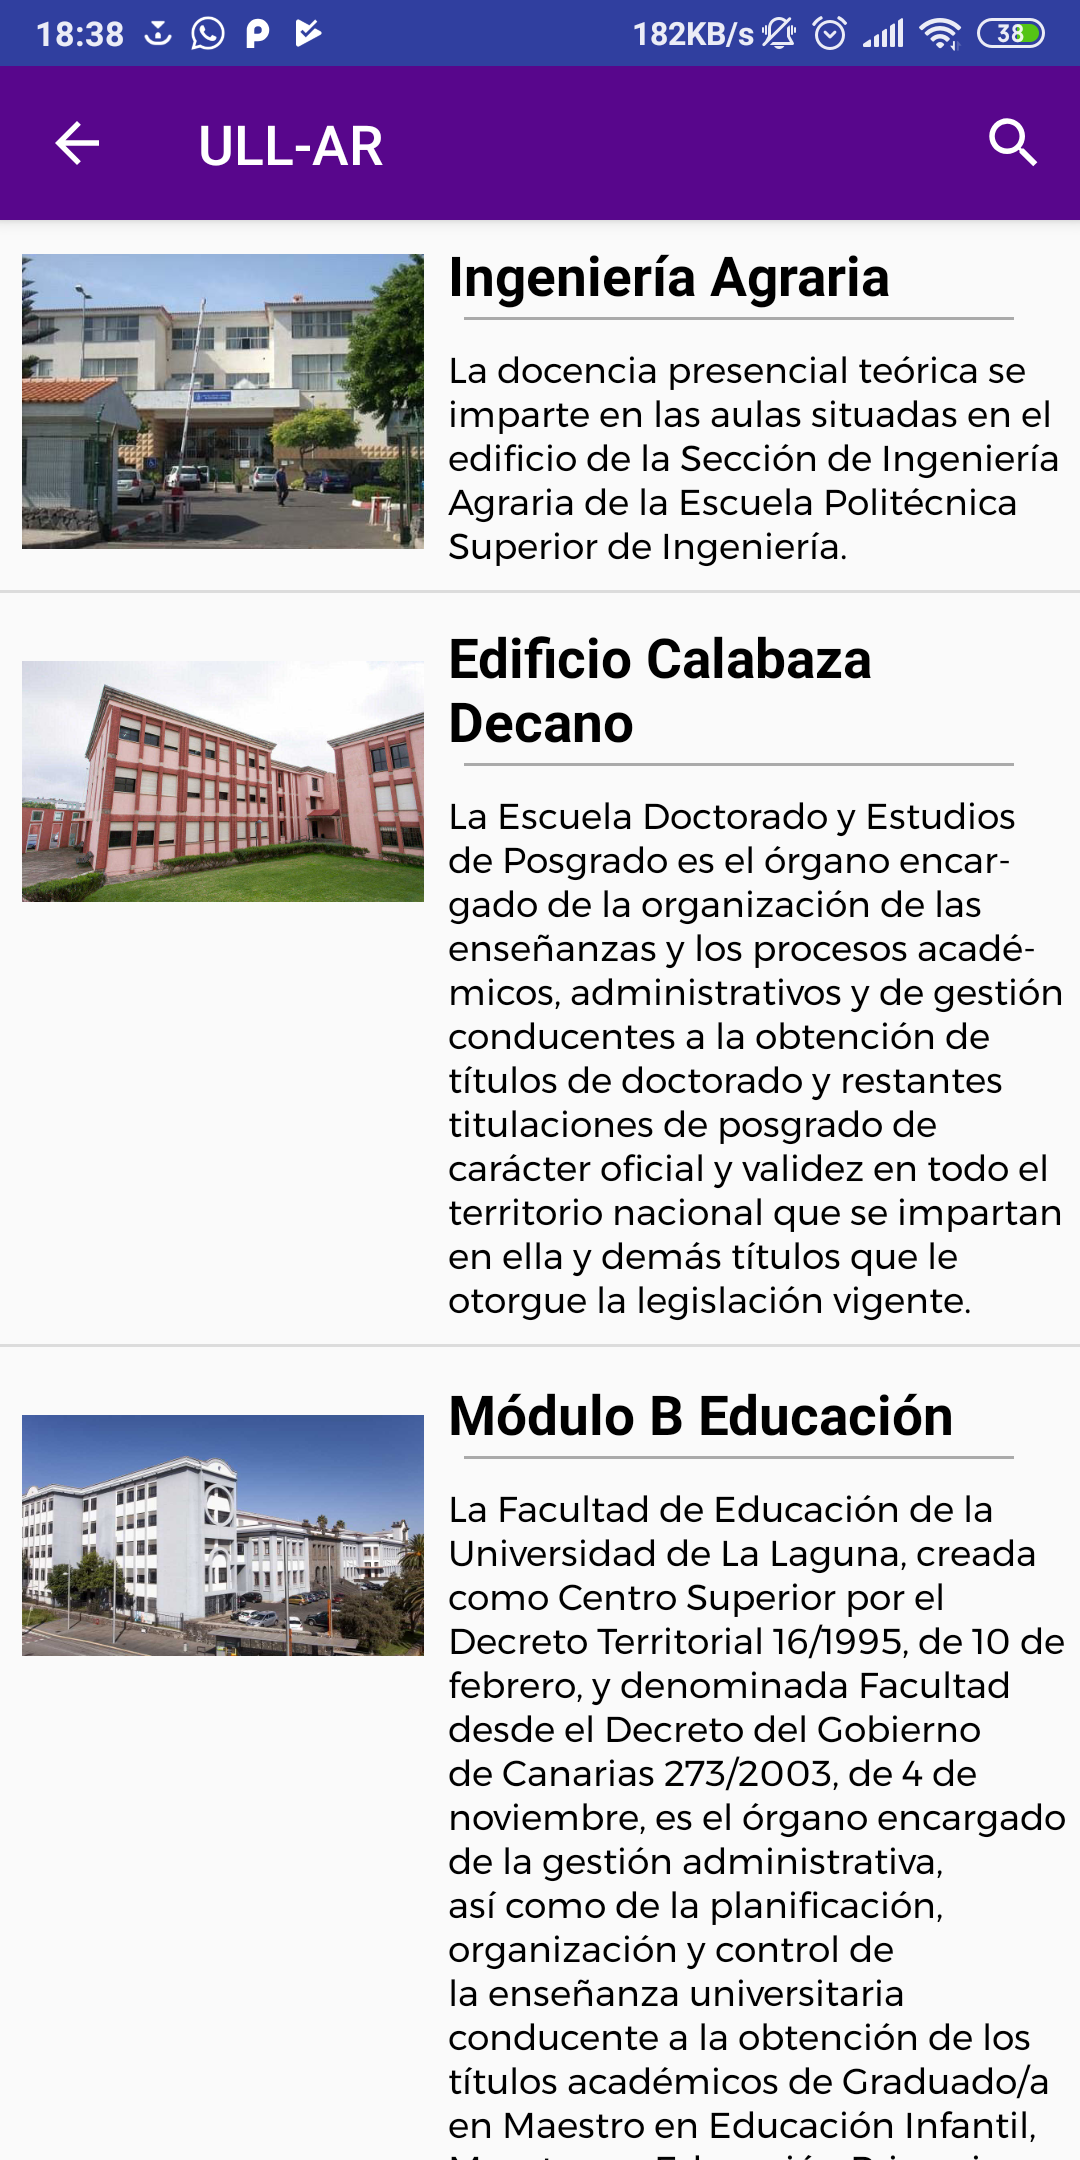
\includegraphics[width=\linewidth]{allSitesApp}
    \caption{Todas las instalaciones ULL.}
    \label{fig:allSitesApp}
    \end{subfigure}
    \hfill%
    \begin{subfigure}[h]{0.35\linewidth}
    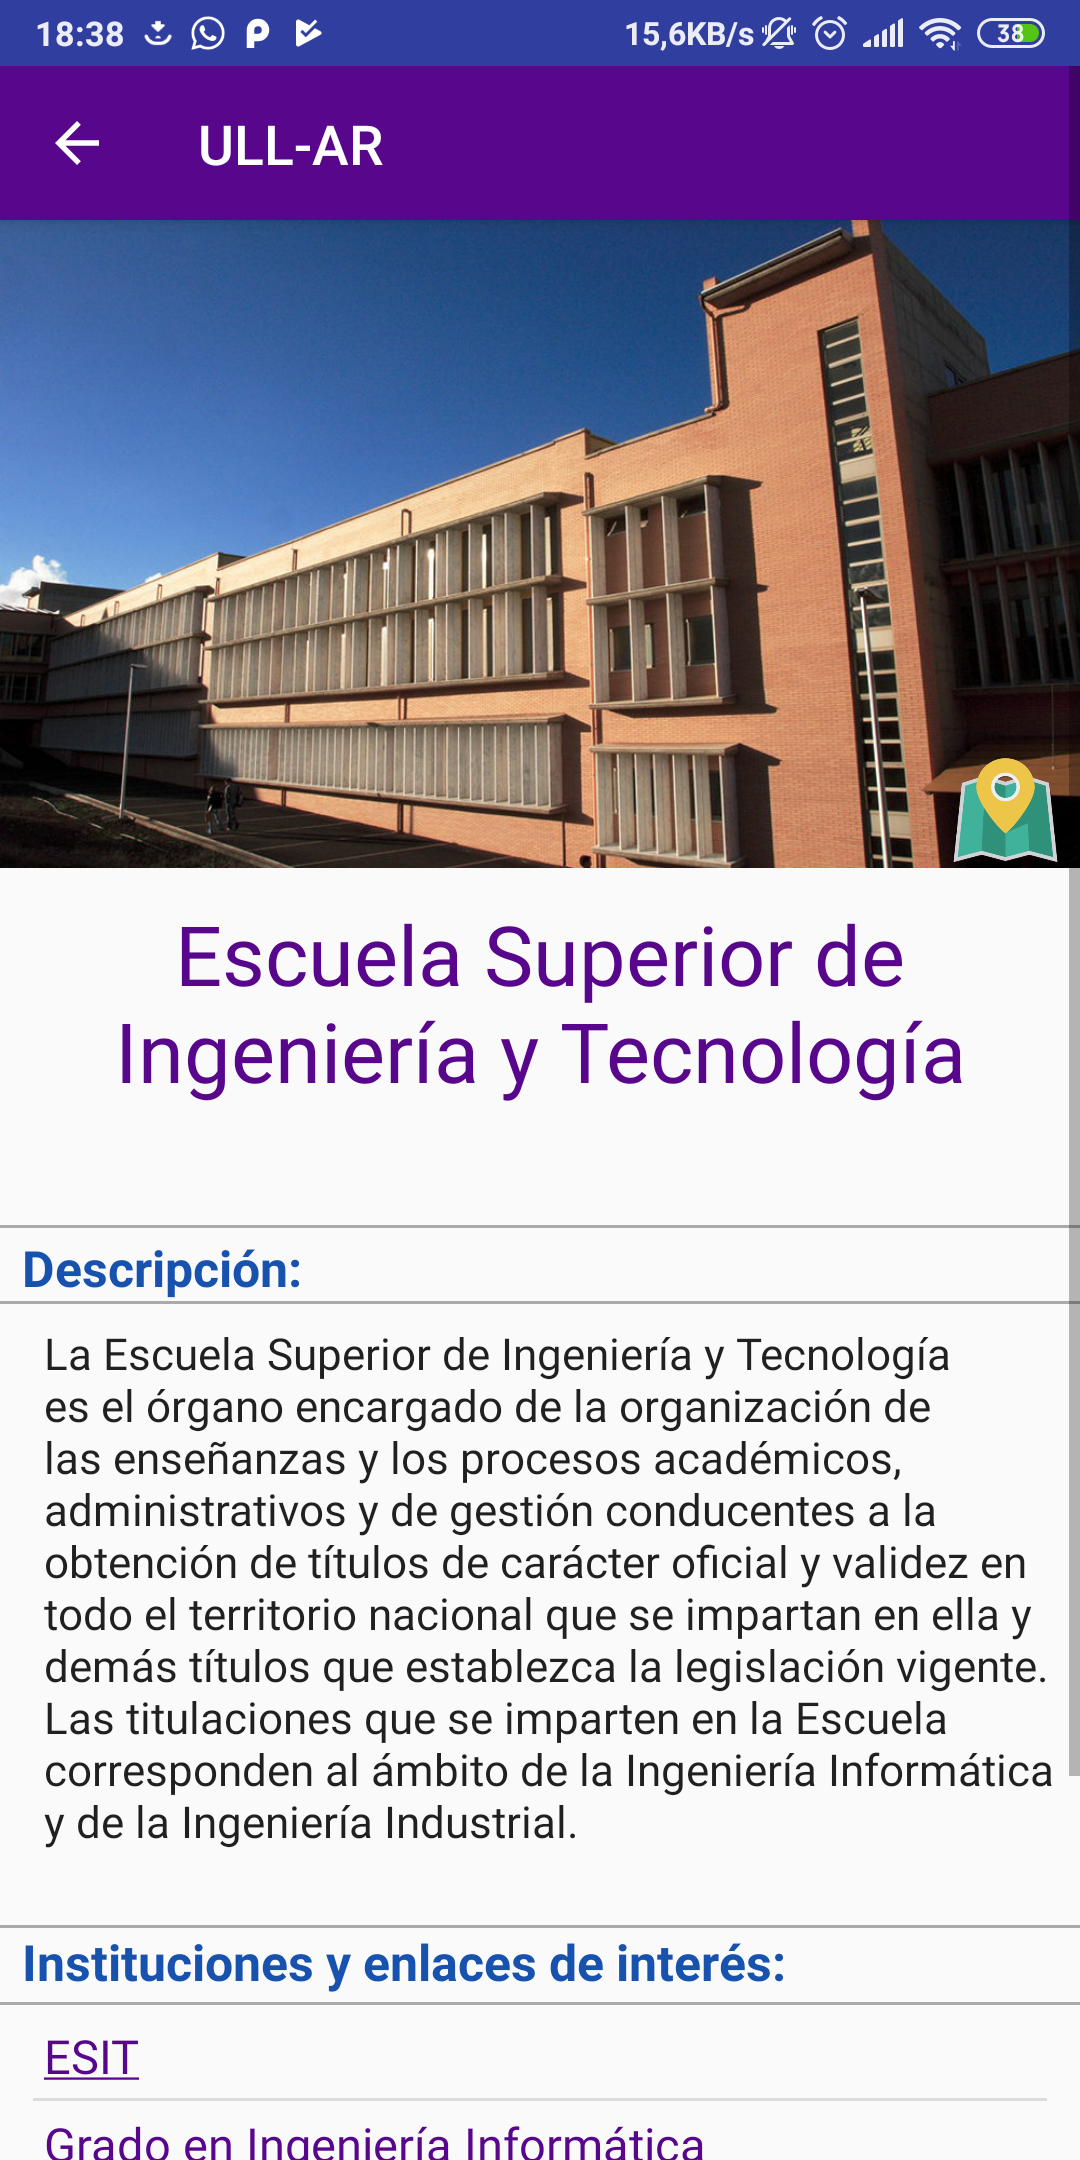
\includegraphics[width=\linewidth]{siteInfoApp}
    \caption{Información de la instalación.}
    \label{fig:siteInfoApp}
    \end{subfigure}%
    \caption{Ventanas de \textit{Todas las instalaciones ULL} e \textit{Información de la instalación} de \textit{ULL-AR}.}
    \hspace*{\fill}%
\end{figure}
 

% \vskip 0.9in

Por último desde el menú podemos acceder a las ventanas de \textit{Configuración} e \textit{Información}.

En la ventana de \textit{Configuración} (véase Figura \ref{fig:settingsApp}) van los ajustes de la aplicación. En ella tenemos la opción para poder configurar si queremos encontrar las instalaciones que se encuentran en el área entre dos circunferencias.

La ventana \textit{Info} (véase Figura \ref{fig:infoApp}) nos muestra información básica de la aplicación como el nombre, versión, correo de contacto, autor y objetivo e información del desarrollo de la aplicación \textit{ULL-AR}. 

\begin{figure}[h]
    \hspace*{\fill}%
    \begin{subfigure}[h]{0.35\linewidth}
    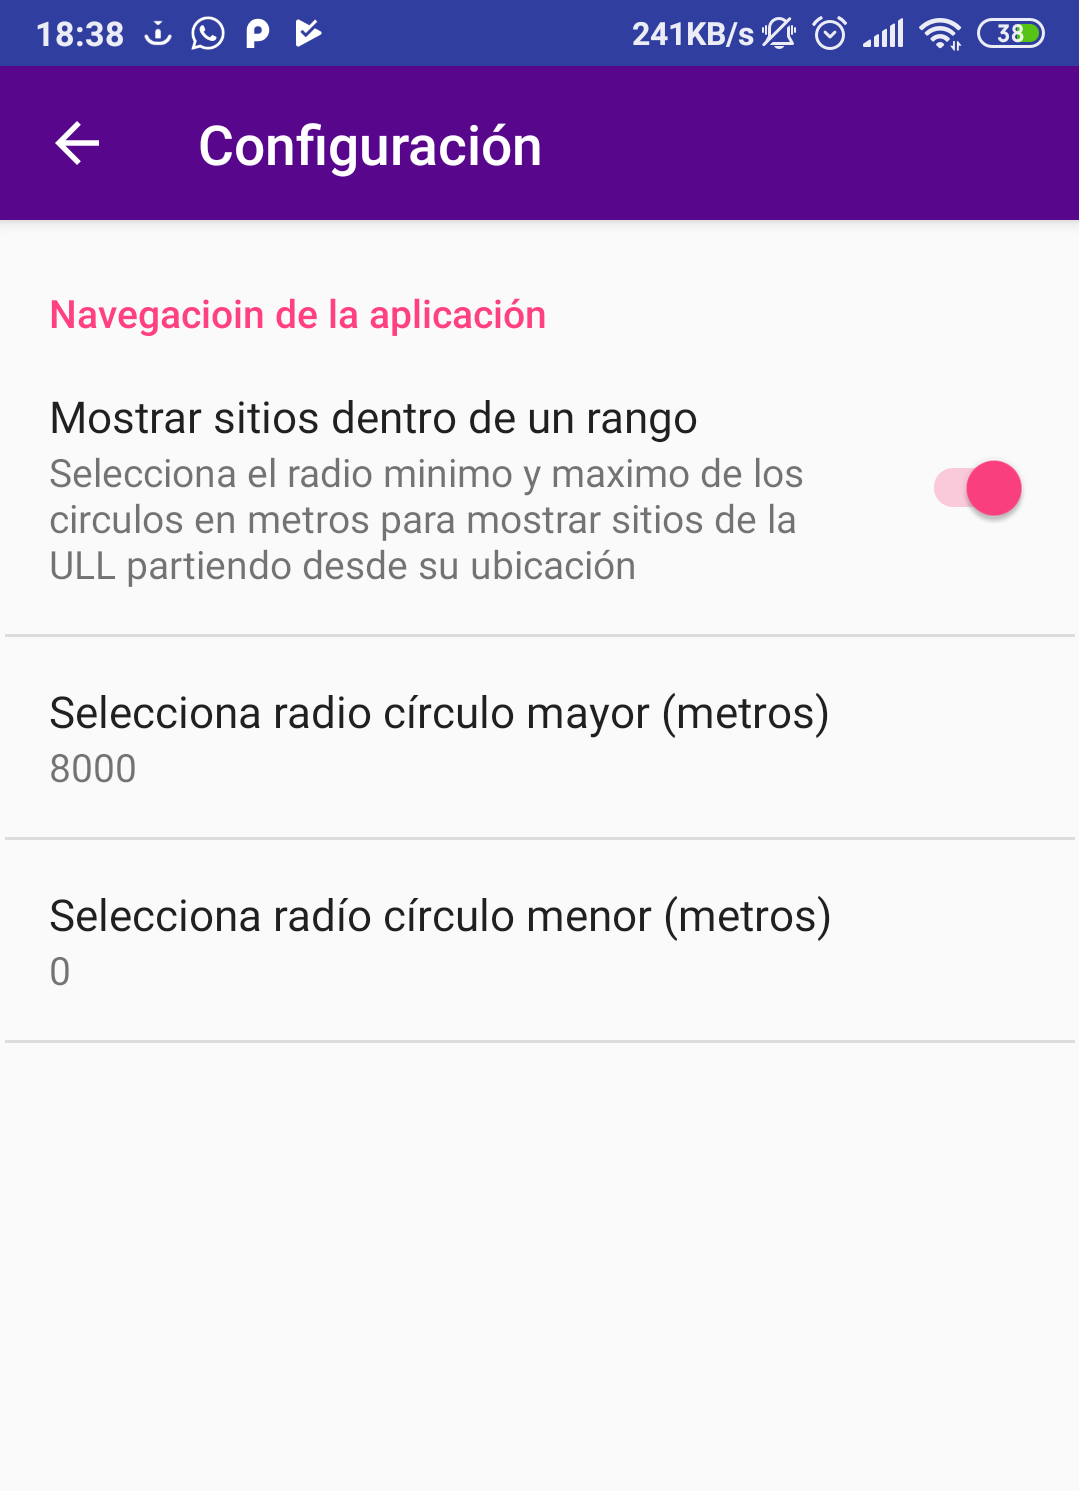
\includegraphics[width=\linewidth]{settingsApp}
    \caption{Configuración.}
    \label{fig:settingsApp}
    \end{subfigure}
    \hfill%
    \begin{subfigure}[h]{0.35\linewidth}
    
\includegraphics[width=\linewidth]{infoApp}
    \caption{Información.}
    \label{fig:infoApp}
    \end{subfigure}%
    \caption{Ventanas de \textit{Configuración} e \textit{Info} de \textit{ULL-AR}.}
    \hspace*{\fill}%
\end{figure}


% subsection  (end)

% -El tfg se realizará en latex
% -Desarrollo en linux
% -Movernos por la universidad
% -Realidad aumentada estudio
% -AR sdk para android 
% -AR por locacizacion
% -Maps
% -Todos las instalaciones universitarios con su locacizacion nombre, des-cripción y enlaces de las instituciones.
% -Splash screen
% -Autentificación con cuenta google de a ULL
% -Ficha de los sitios
% -Posibilidad de cerrar sesión 
% -Pestaña de información de la aplicación
% -Una pestaña de configuración 
% -Back-end, servidor y base de datos en la nube para mayor facilidad en las pruebas 
% -



% \section{Implementación}
% \section{Desarrollo}










% \lstset{numbers=left, stepnumber=2, frame=single,}
% \lstinputlisting[float, floatplacement=H, caption={La clase \textit{Arrival} donde quedan contenidos los datos de cada llegada.}, label={code:arrival}]
% {listings/Arrival.java} %% LISTING


